\documentclass[12pt]{article}
\usepackage{graphicx}
\usepackage{amsmath}
\usepackage{booktabs}
\usepackage{hyperref}
\usepackage{geometry}
\usepackage{float}
\geometry{a4paper, margin=1in}

\title{A Deep Dive into NBA All-Star Selections and Player Utilization: Performance, Fairness, and Efficiency}
\author{Stats 140XP Group 12 \\ Tyler Chia, Ray Min, Kevin Liu, Darion Phan, Chinmay Varshneya, Ian Zhang}
\date{\today}

\begin{document}
\maketitle

\begin{abstract}
NBA player evaluation is typically subjective, but a player's minutes and whether or not they are selected as an All-Star is not. We hope to better evaluate NBA players and understand if they are "deserving" of the recognition they recieve in the form of minutes and awards. To test this hypothesis, we used NBA data dating back to 1947 found on Kaggle. Logistic regression, random forests, and other models were created to see if the player's All-Star selection and minutes played could be predicted. Once these models were created for both the All-Star selection and minutes played, we compared their the outputs and decided which models were the best for classifying or predicting. It was found that we are able to predict All-Star selection to a relatively high accuracy using season statistics alone, but cannot perfectly predict All-Stars. For the expected minutes played, we found which players were being overutilized and underutilized. Our findings show that we can predict All-Star selection and the expected minutes played for players relatively well, but cannot perfectly predict it. The next steps that could be taken for All-Star selection would be to compare the All-Star vote count by years and compare the season statistics of players that were nominated. The next steps that could be taken for predicting the expected minutes played would be to see how different coaches or offensive systems change players' usage and other statistics because coaches are who determine which players are playing.
\end{abstract}

\section{Introduction}
With the NBA season in full swing, our team is diving into two of the biggest questions in the league right now: Who should truly be an All-Star, and which players are either underutilized or overutilized on their respective teams? These looming questions in the NBA have significant implications not only for individual player recognition and contracts but also for overall team performance and efficiency on the court.
The All-Star Game is meant to showcase the best talent in the league, and every year there are many snubs and questionable selections. The current voting system is composed of three key components: fan voting, media voting, and coaches’ selections. Fan voting accounts for 50\% of the vote, while media voting and coaches’ selections each account for 25\%. This system can introduce significant bias, as popularity and market size heavily influence fan votes. For example, in the 2017 season, Zaza Pachulia, a player not known for being at an All-Star level, received the fifth-most votes in the Western Conference, surpassing notable players such as Anthony Davis, Chris Paul, and Damian Lillard. This was largely due to his team at the time, the Golden State Warriors, being one of the best teams in the league with a massive fan market. Such biases in fan voting have caused significant controversy, as they can lead to less statistically deserving players making the cut. Meanwhile, coaches vote to select All-Star reserves, often prioritizing veteran experience and team success over statistical excellence. Our analysis aims to determine who should genuinely be an All-Star based on an objective assessment of statistical performance. For example, we believe that players such as LaMelo Ball and Domantas Sabonis, who have been incredibly impactful for their teams and have outstanding statistics, deserve All-Star recognition. By leveraging machine learning algorithms, we seek to provide a robust, data-driven approach to identifying the most deserving players.

Beyond individual accolades, team performance is deeply affected by how players are utilized. Are certain players not getting enough minutes despite their efficiency and impact? Conversely, are some players playing too many minutes relative to their production, potentially hurting their teams? Team success depends on how well players are utilized within their respective systems. Some players may not be receiving enough playing time despite their high efficiency and overall impact, whereas other players may be logging excessive minutes while delivering subpar performances. Beyond on-court performance, player utilization also directly impacts a team’s contract decisions. Teams often allocate significant financial resources to their top players, sometimes leaving less than half of their salary cap to fill the roster with role players. The way teams balance funds between contracts is a crucial yet often overlooked aspect of roster management. Underutilized players may not receive contract extensions or deals that reflect their true value, while overutilized players may be rewarded with disproportionate contracts.
To address these inefficiencies, we will analyze advanced metrics such as Points per Minutes and Assist-to-Turnover Ratio. Additionally, we will examine optimal minute distribution by considering fatigue effects, injury risk, and lineup efficiencies. By doing so, we aim to provide data-driven insights on how teams can maximize their potential and efficiency.
Through our analysis, we seek to highlight inefficiencies in both team operations and the current NBA All-Star voting system. By applying data-driven methodologies, we hope to bring greater objectivity to player recognition and team management, ensuring that players are evaluated based on their actual contributions rather than subjective biases. Ultimately, our findings will serve as a foundation for more informed decision-making in lineup optimization, contract structuring, and overall team strategy.

\section{Literature Review}

Sports data science, specifically in major league American sports, is focused on predictive analytics. As such, papers commonly employ a wide variety of machine learning algorithms in order to accurately predict player statistics and overall game outcomes. Notable studies in this realm include those by Jingru Wang and Qishi Fan which applied machine learning to player All-star selection and playoff qualification \cite{wang2021}. Other common areas of study in the NBA include the application of more complex multilayer perceptron algorithms and deep neural networks to regular season game outcomes \cite{georgievski2021}. Studies that employ various algorithms for NBA prediction are plentiful \cite{wang2023}, and therefore aside from papers that innovate when it comes to the models (see DNNs), the most relevant area of study is feature selection. Common findings point to using defensive statistics as well as common indicators such as efficiency and points per game. Various studies all point to similar optimal feature sets, upon which several common models are run including Random Forest, Bayesian Ridge, and XGBoost to reach a modest degree of accuracy \cite{alonso2024}. Our paper will attempt to build on this existing body of work with regard to player performance, specifically as it pertains to accolades and roster management.  

\section{Research Questions}

We’re tasked with creating a larger research question and the questions in this section are used to address the larger research question. The overarching theme of these questions is about player on-court impact. Essentially, “Can we compare the impact of individual players in the team game of basketball?” Below are the specific research questions that can help get us there. 

\begin{itemize}
    \item Can we predict NBA All-Star selections using historical and current season performances? Are some players more deserving than others?
    \item Does the data suggest that some players are underutilized or overutilized? Should certain players get more or fewer minutes?
\end{itemize}

\section{Data}
The data included both counting statistics (points, rebounds, assists, etc) and advanced metrics (expected three pointers per game, etc.). With two different research questions, we utilized different data cleaning techniques to tailor the data to answer each question.

For the first question, we start with a dataset including columns: Player, Season, Points, Personal Fouls, Turnovers, Blocks, Steals, Assists, Defensive Rebounds, Offensive Rebounds, Free Throw Attempts, Free Throws Made, Two-Point Attempts, Two-Pointers Made, Three-Point Attempts, Three-Pointers Made, Field Goals Attempted, Field Goals Made, Minutes Played, Games Started, Games Played, and All-Star. The feature abc only has data collected from the 1982 season up to the 2024 season, so we only consider seasons in this range. We are interested in using a player’s performance in a given season to predict the binary class All-Star which represents whether a player will be selected as an All-Star (or not). Each row represents a single player’s performance in a single season, adding up to a total of 18,803 rows, with 1081 (Player, Season) combinations selected as All-Stars. There are proportionally much greater non-All-Stars in the dataset than All-Stars, which we handle using random undersampling of non-All-Stars. This means the final dataset used for training contains all 1081 All-Star inputs as well as 4000 randomly sampled non-All-Star inputs (for a final dataset of size 5081). This ensures that the dataset is balanced which is very important for training classification models.

For the second question, we employed the same data set titled as for the first question. However we had to approach the data from a slightly different perspective than done for the first research question. To glean some initial understanding of the dataset, we employed the Pandas describe method to view the summary statistics of our dataframe. After which, we had to conduct some light feature engineering to make the data more apt for our methodology. We added several features which described player efficiency including ppm (points per minute), fg\_pct (field goal percentage), x3p\_pct (three point percentage), x2p\_pct (two point percentage), ft\_pct (free-throw percent, and ast\_tov (assist to turnover ratio). These additions simply involved manipulating the existing variables. Since our question looks to understand how many minutes a player should be receiving in a game, we had to normalize the statistics based on volume as that scales with minutes played. Volume, as seen in the above changes, is mostly concerned with the number of shots taken. The last new feature added was mpg (minutes per game) which is the variable we will look to predict in our final model. 

\section{Exploratory Data Analysis}

\begin{figure}[h]
    \centering
    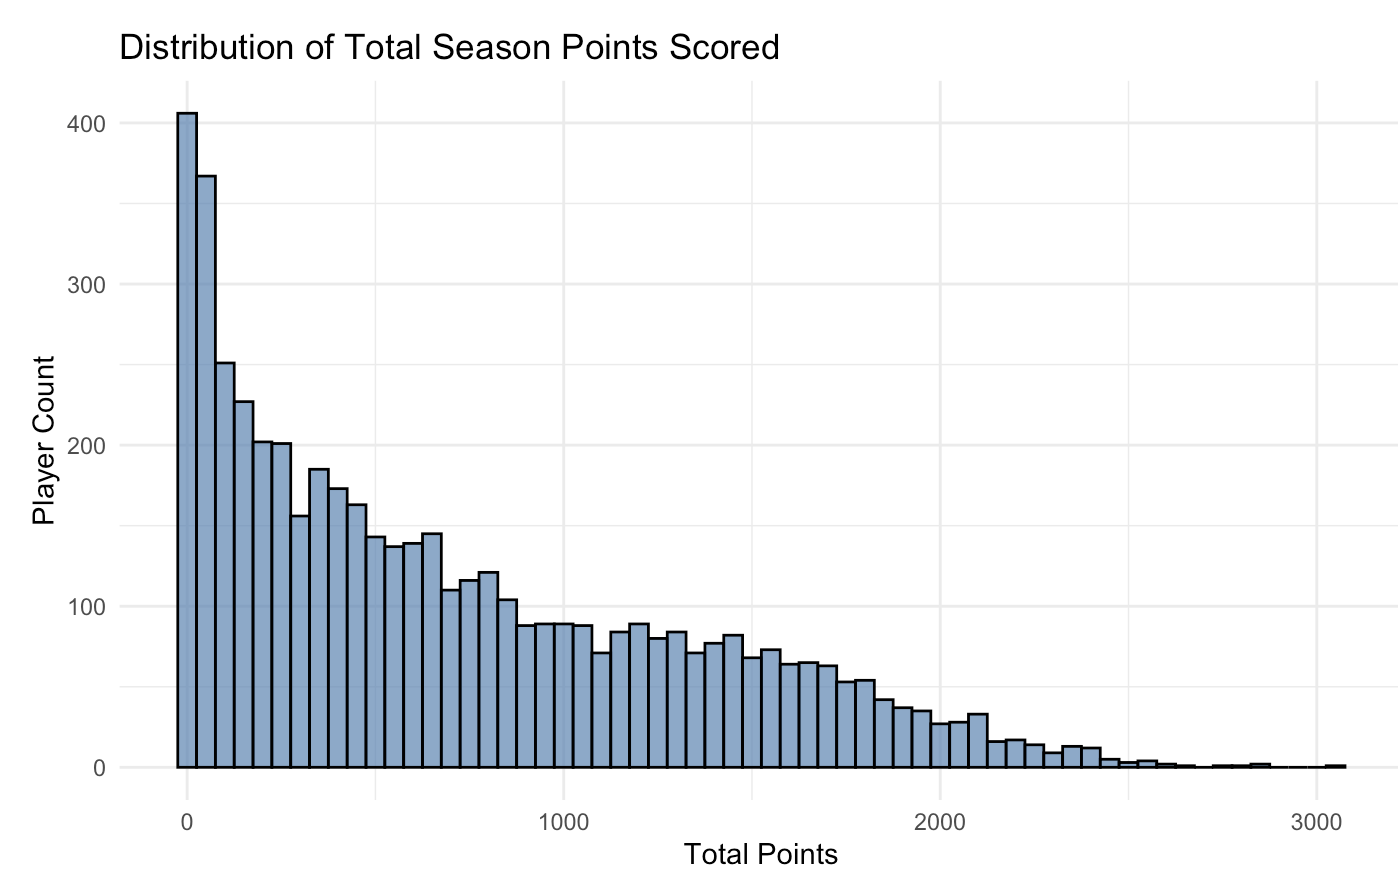
\includegraphics[width=0.8\textwidth]{EDA_HISTOGRAM.png}
    \caption{Histogram displaying the distribution of total points scored by players in an NBA season across all players from 1947-Present.}
    \label{fig:points_distribution}
\end{figure}

The histogram above displays the distribution of total points scored by players in an NBA season. We see that many players score a very low amount of points. As we move right along the x-axis, we see that the number of players gets lower and lower in the higher point totals. This suggests that the majority of players score fewer points in a season, while only a select few achieve elite-level scoring numbers exceeding 2,000 points. The long tail on the right side of the histogram represents the league’s top scorers, who contribute a significantly higher number of points compared to the average player.

\begin{figure}[H]
    \centering
    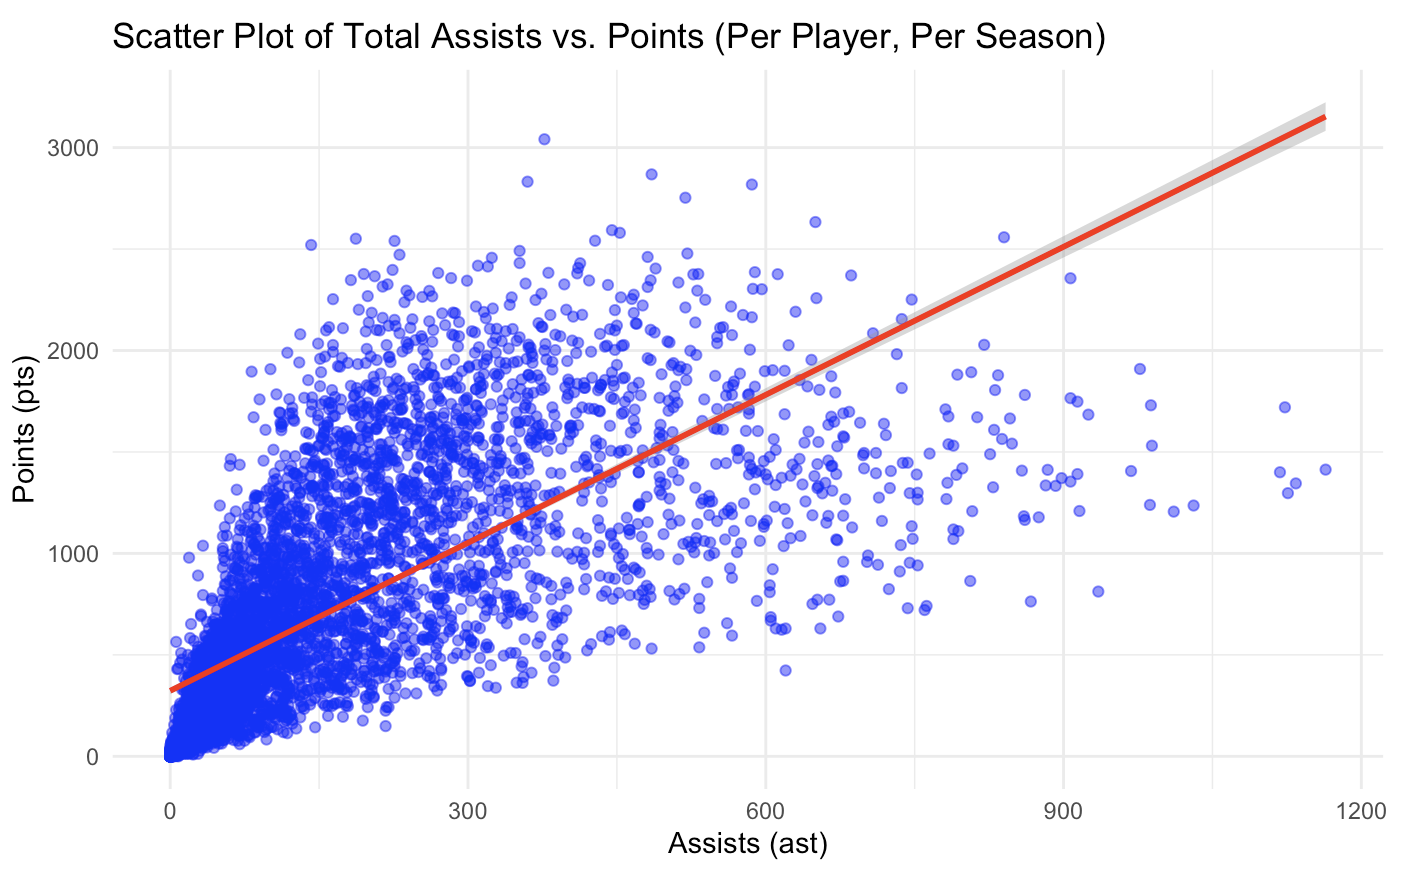
\includegraphics[width=0.8\textwidth]{EDA_SCATTERPLOT.png}
    \caption{Scatter plot showing the relationship between total assists and total points per season. The correlation is positive.}
    \label{fig:assists_vs_points}
\end{figure}

Next, we took a look at if there is any correlation between the total assists and total points a player accumulates in a single season. Each point represents an individual player’s season totals. We notice that there is a positive correlation between the total number of assists and points, showing that players who record a high number of assists also tend to score more points. This makes sense because a player who is accumulating a high number of either points or assists is probably playing a high number of minutes per game, leading to them having more opportunities to score and/or assist. We also see a similar trend as the histogram prior. There is a high density of players that have low point and assist totals, and fewer players with high point and assist totals. Lastly, we see that there are some outliers with extremely high assist and point totals, likely representing stars who contribute significantly to their team.

\begin{figure}[H]
    \centering
    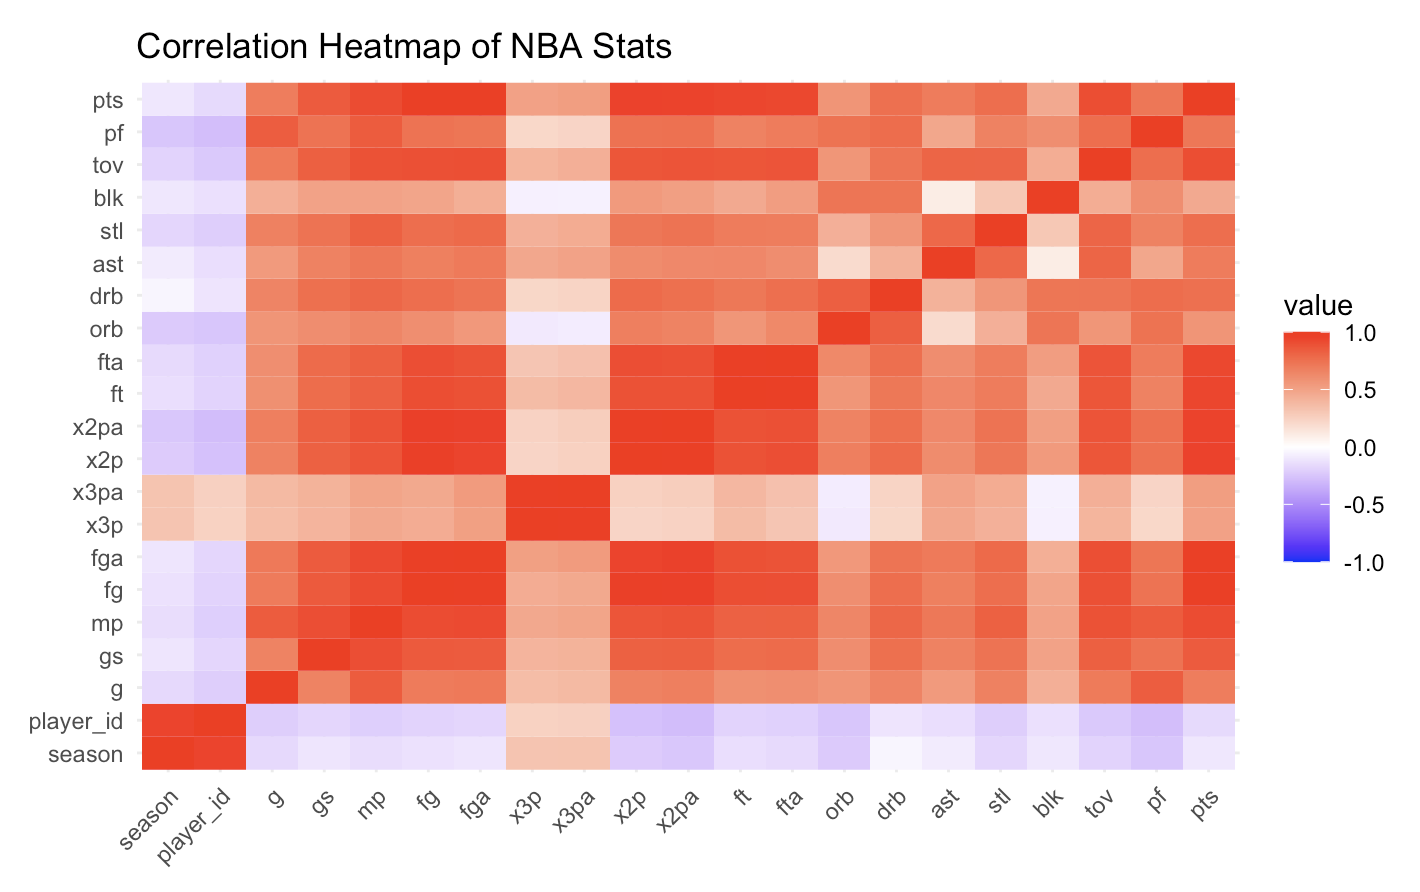
\includegraphics[width=0.8\textwidth]{EDA_HEATMAP.png}
    \caption{Correlation heatmap displaying relationships between various player statistics such as points, field goals, assists, and turnovers.}
    \label{fig:correlation_heatmap}
\end{figure}

The correlation heatmap above indicates strong positive correlations between points (pts) and field goals made (fg), suggesting that higher-scoring players tend to make more shots. Assists (ast) and points (pts) also shows a positive relationship, highlighting players who contribute both in scoring and playmaking. Defensive rebounds (drb) and blocks (blk) are also positively correlated, most likely indicating defensive-focused big men who grab lots of rebounds and block shots close to the rim. Lastly, turnovers (tov) and points (pts) have a high correlation, indicating that players who score the ball more also turnover the ball at a higher rate. This can be due to the fact that the players who score more have the ball more often, leading to more possibilities for turnovers. 

Afterwards, we progressed to feature selection. This meant determining which variables are most highly correlated with a player’s quality of play. In order to answer this question, we referred back to our previous work with all-star selection. Our rationale was that the most important features in determining whether a player is an all-star are, by virtue of the award, also the most important in determining if a player is “good” or not. Therefore we ran a random forest model for all-star prediction and then referred to the fitted attribute feature\_importances\_. The results are as follows: 

\begin{figure}[H]
    \centering
    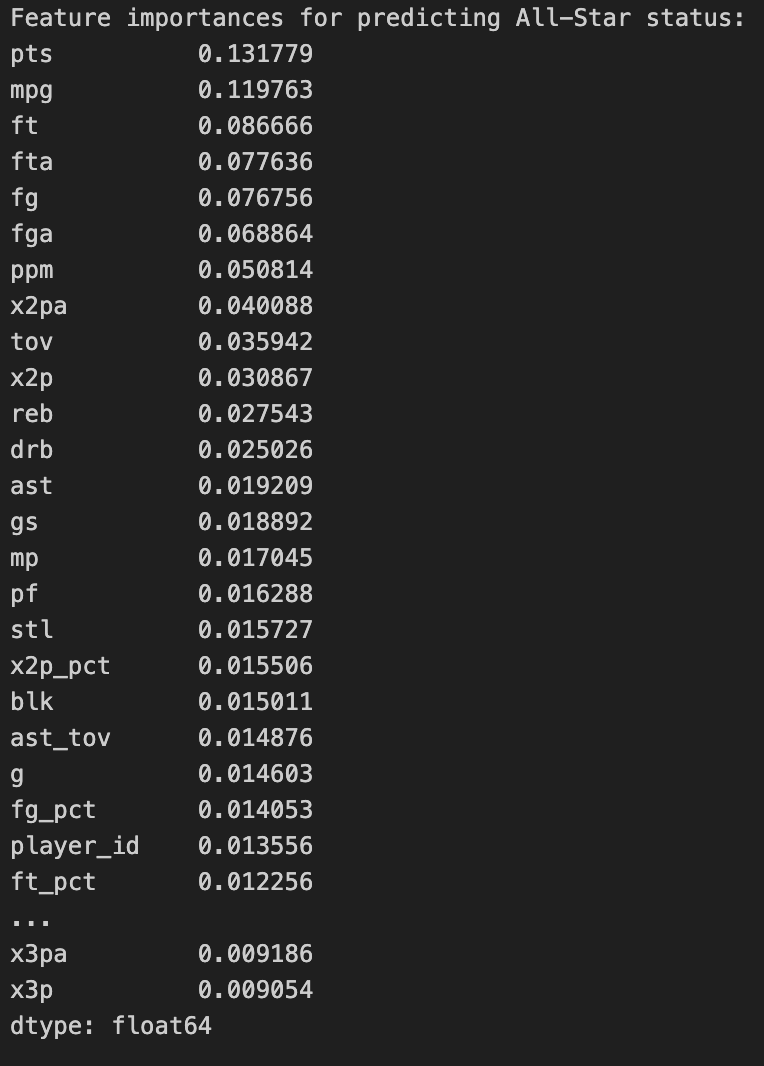
\includegraphics[scale = 0.5]{EDA_FEATURE_SELECTION.png}
    \caption{Feature importance plot from a Random Forest model predicting All-Star selections. Points scored, field goals made, and free throws made are the most influential features.}
    \label{fig:feature_importance_allstar}
\end{figure}

After removing highly correlated features (as well as mpg), we were left with our final variables for our expected minutes model: 'pts', 'ft', 'fta', 'fg', 'fga', 'ppm', 'x2pa', 'tov', 'x2p', 'reb', 'drb',  and 'ast'.

\section{Models and Methods}
\subsection{Predicting All-Star Selection}
\subsubsection{Logistic Regression:} The first model we used to answer this question was a logistic regression model. This was the simplest model to train and implement and takes into account 12 of the 19 predictors. As the original 19 predictors had multicollinearity, we had to reduce the number of variables using stepwise regression, choosing our model using AIC. Ultimately, we ended up with an accuracy score of 92.22\% using logistic regression. 

\begin{figure}[h]
    \centering
    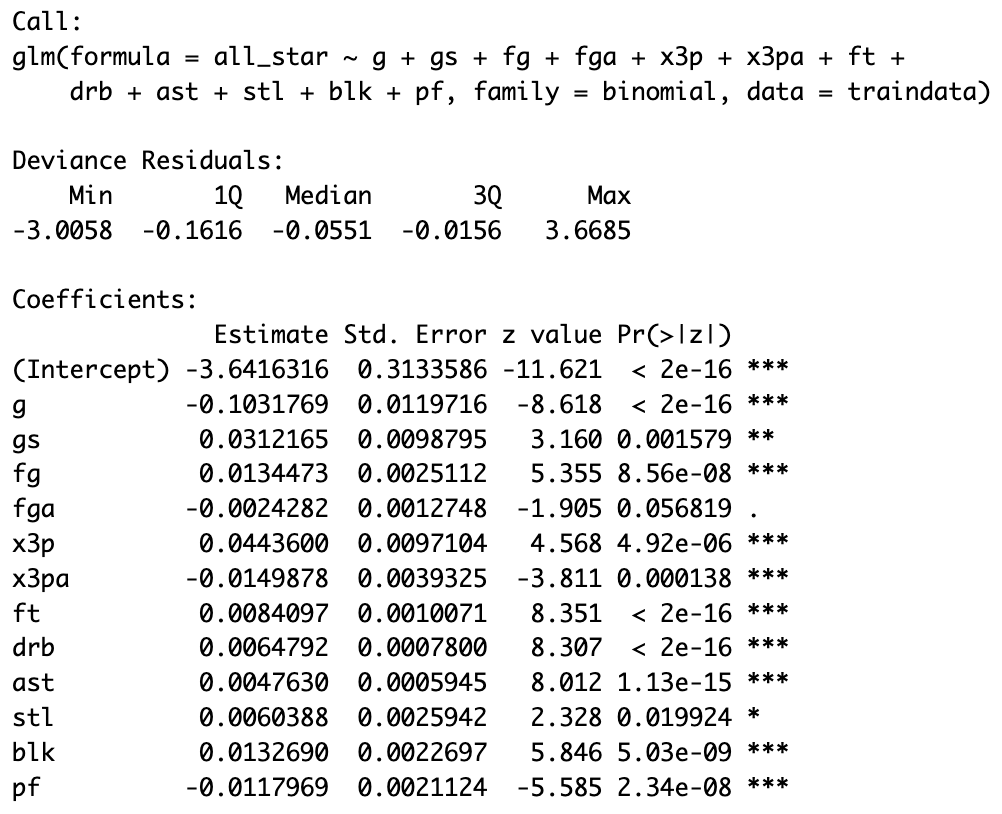
\includegraphics[width=0.8\textwidth]{MM_AS_FUNCTION_CALL.png}
    \caption{Coefficients of the logistics regression model}
    \label{fig:decision_tree_confusion_matrix}
\end{figure}

\begin{table}[h]
    \centering
    \begin{tabular}{c|cc}
        \toprule
        \textbf{Prediction} & \multicolumn{2}{c}{\textbf{Reference}} \\
        \midrule
        & 0 & 1 \\
        \hline
        0 & 753 & 44 \\
        1 & 35 & 184 \\
        \bottomrule
    \end{tabular}
    \caption{Confusion matrix of the logistic regression model.}
    \label{tab:confusion_matrix}
\end{table}

\subsubsection{Tree Models} The second (family of) models we used to answer the question was tree algorithms. Specifically we tested both a decision tree and a random forest. Decision trees classify by recursively splitting the feature space based on thresholds that maximize information gain, leading to leaf nodes that assign class labels. Training on the All-Star dataset, we obtained the following tree:

\begin{figure}[h]
    \centering
    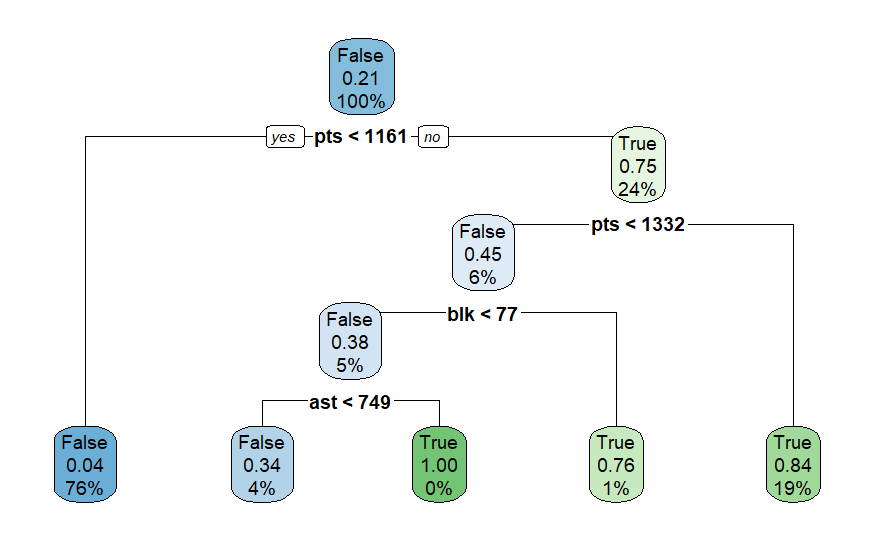
\includegraphics[width=0.8\textwidth]{MM_AS_TREE_DIAGRAM.png}
    \caption{Diagram of the decision tree.}
    \label{fig:random_forest_confusion_matrix}
\end{figure}

\begin{table}[h]
    \centering
    \begin{tabular}{c|cc}
        \toprule
        \textbf{Prediction} & \multicolumn{2}{c}{\textbf{Actual}} \\
        \midrule
        & \textbf{True} & \textbf{False} \\
        \hline
        \textbf{True}  & 754  & 53  \\
        \textbf{False} & 46   & 163 \\
        \bottomrule
    \end{tabular}
    \caption{Confusion matrix for the decision tree.}
    \label{tab:decision_tree_confusion_matrix}
\end{table}

The decision tree splits the feature space on player statistics Points, Blocks, and Assists. Notably, players with a high number of points, blocks and assists in a season are All-Stars. The decision tree achieves 90.26\% accuracy on testing data.

Random forests classify using bagging, where multiple decision trees are trained on random subsets of the data and features, then their predictions are aggregated. Training on the All-Star dataset, we obtained the following feature importance plot for the forest:

\begin{figure}[H]
    \centering
    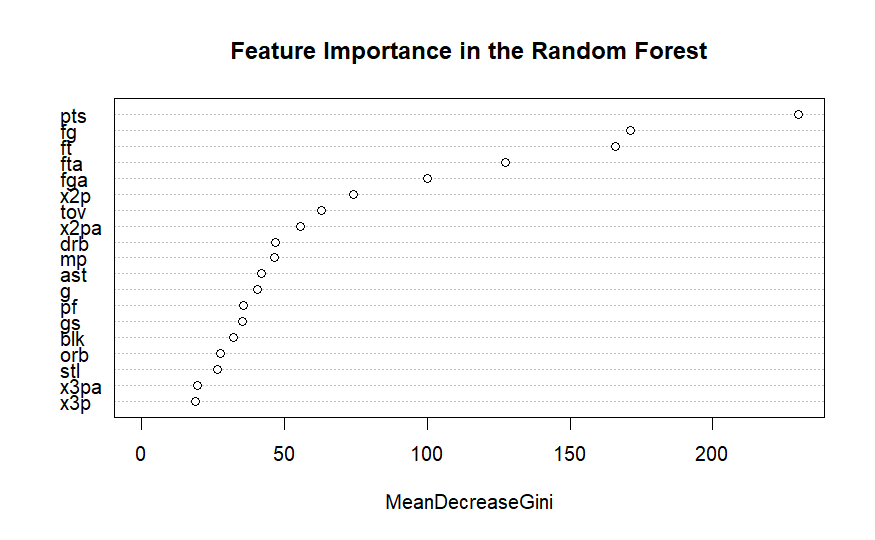
\includegraphics[width=0.8\textwidth]{MM_AS_TREE_IP.png}
    \caption{Feature Importance plot of the random forest model.}
    \label{fig:neural_network_architecture}
\end{figure}

The feature importance plot indicates the most influential features of the dataset are Points, Field Goals Made, and Free Throws Made. The random forest achieves 92.03% accuracy on testing data.

\begin{table}[h]
    \centering
    \begin{tabular}{c|cc}
        \toprule
        \textbf{Prediction} & \multicolumn{2}{c}{\textbf{Actual}} \\
        \midrule
        & \textbf{True} & \textbf{False} \\
        \hline
        \textbf{True}  & 754  & 44  \\
        \textbf{False} & 46   & 172 \\
        \bottomrule
    \end{tabular}
    \caption{Confusion matrix for the random forest}
    \label{tab:decision_tree_confusion_matrix}
\end{table}

The decision tree and random first largely perform the same on the All-Star prediction task, with the random forest achieving slightly higher testing accuracy. Though both models learn different features for determining All-Star selections, they share the selection of Points as a particularly influential statistic.

\subsubsection{Neural Network}

The third model we used to answer this question was a neural network. This process is complicated and takes into account fan, established media, coach, and player voting with basketball statistics playing an indirect role in the selection. The neural network allows us to fit a function to this complex relationship. The inputs to this neural network were the 19 counting statistics and there was one output. There is one hidden layer with eight nodes. 

\begin{figure}[h]
    \centering
    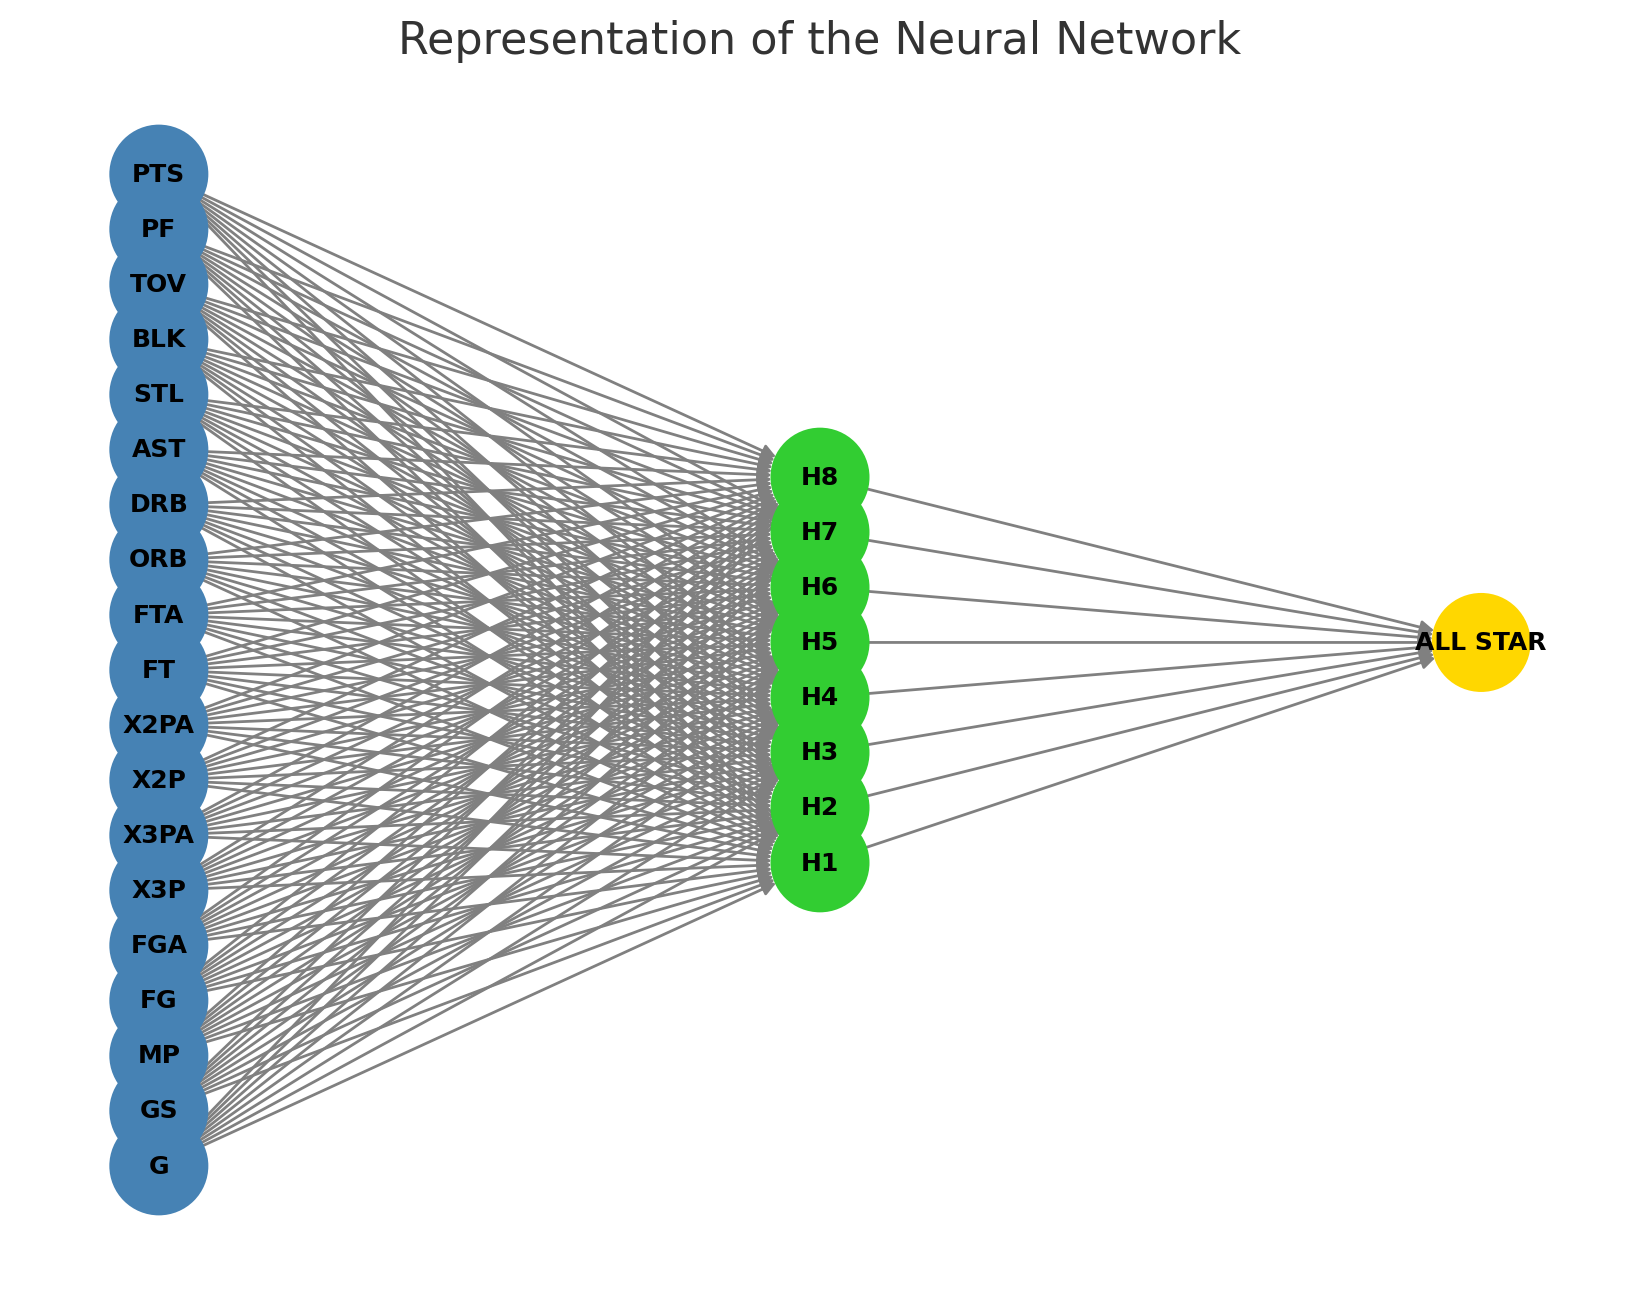
\includegraphics[width=0.8\textwidth]{AS_MM_NN_GRAPHIC.png}
    \caption{Representation of the neural network}
    \label{fig:minutes_difference_distribution}
\end{figure}

\begin{table}[h]
    \centering
    \begin{tabular}{c|cc}
        \toprule
        & \textbf{Absolute} & \textbf{Per-Game} \\
        \midrule
        \textbf{Small} & 0.9237561 & 0.7888692 \\
        \textbf{Large} & 0.9647753 & 0.9422388 \\
        \bottomrule
    \end{tabular}
    \caption{Accuracy compared across different dataset sizes and type of statistic}
    \label{tab:absolute_vs_pergame}
\end{table}

This neural network was created with balanced data and imbalanced data. Absolute season statistics and per-game season statistics were used. All combinations of these modifications were used, meaning this neural network was made using four different datasets. Each dataset was used 50 times to get a better estimate of the neural network’s accuracy.

This could be due to the number of non-All-Stars in the imbalanced data that skewed the accuracy, but we can still analyze the relative accuracies between the combinations. The absolute statistics on the larger dataset had a higher accuracy than the per-game statistics on the larger dataset. Similarly, the absolute statistics on the smaller dataset had a higher accuracy than the per-game statistics on the smaller dataset. Then we see that a player’s absolute statistics are better than their per-game statistics in deciding who the All-Stars will be.

\subsection{Player Utilization Analysis}
Using the select features described above, we ran the default version of several common machine learning models (linear regression, decision tree, random forest, support vector regressor, gradient boosting regressor) with the target prediction variable being mpg or minutes per game. Effectively, we were using the most important variables for determining player quality to gauge  the amount of minutes a player was expected to play in a game based on their efficiency. We tested model accuracy using their actual minutes per game and used root mean squared error as well as the coefficient of determination to compare the models. The gradient boosting regression algorithm performed best in both metrics. 

\begin{figure}[H]
    \centering
    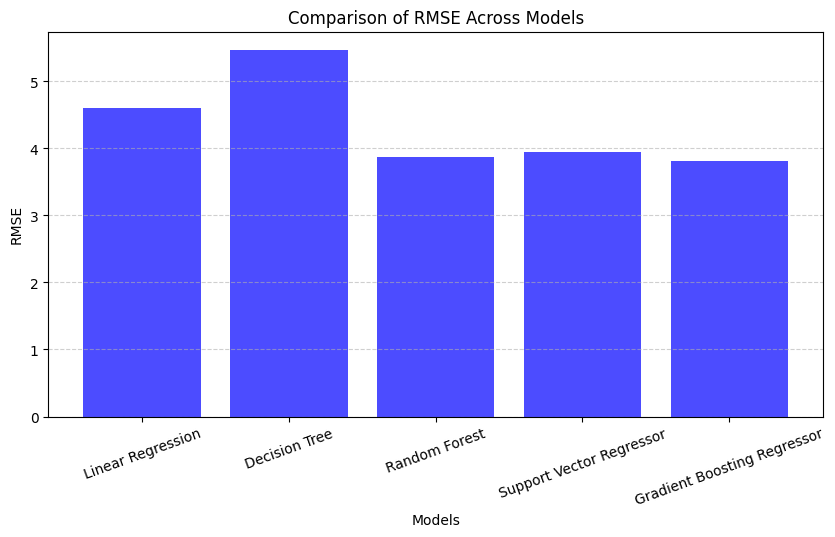
\includegraphics[width=0.8\textwidth]{MM_EP_RMSE.png}
    \caption{Bar plot displaying the RMSE for different models}
    \label{fig:team_utilization}
\end{figure}

\begin{figure}[H]
    \centering
    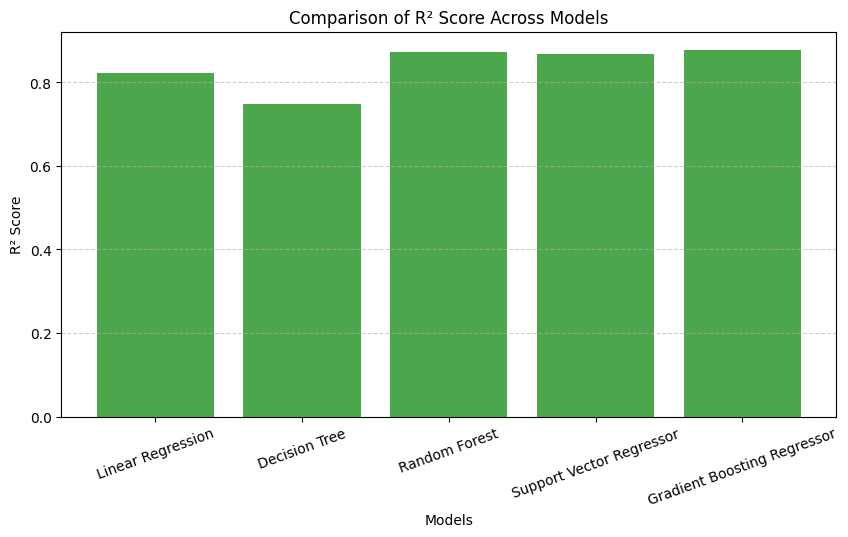
\includegraphics[width=0.8\textwidth]{MM_EP_R2.png}
    \caption{Comparison of $R^2$ for different models.}
    \label{fig:model_comparison}
\end{figure}

As such, we selected the gradient boosting model as our final model and used it to answer our question of player utilization. This entailed calculating the difference between the “expected” and “actual” minutes played per game by every player in our dataset. We conducted some basic exploration of this metric to ensure it was appropriate.

\begin{figure}[H]
    \centering
    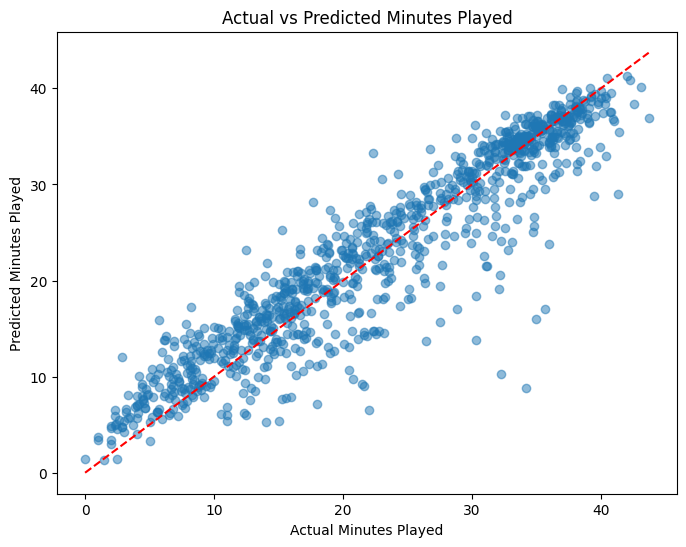
\includegraphics[width=0.8\textwidth]{MM_EP_AVPMP.png}
    \caption{Scatter plot of actual versus predicted minutes played}
    \label{fig:feature_selection}
\end{figure}

\begin{figure}[H]
    \centering
    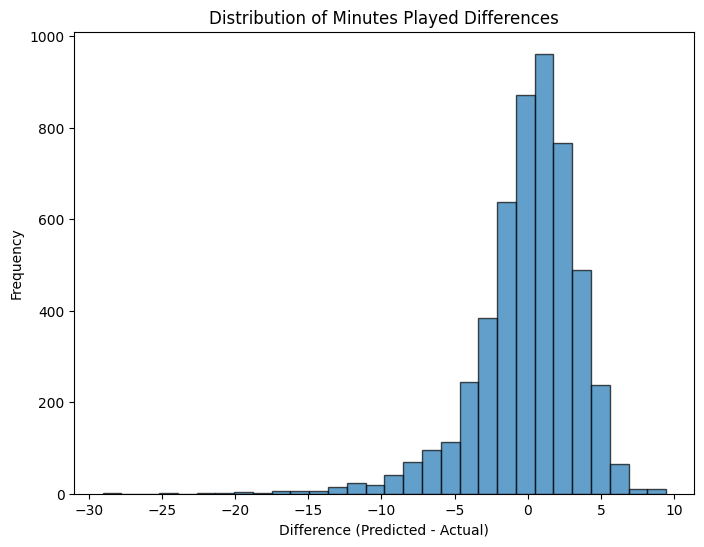
\includegraphics[width=0.8\textwidth]{MM_EP_DMPD.png}
    \caption{Histogram of the difference between predicted and actual minutes played}
\end{figure}
As should be expected, the difference is centered around zero and is roughly normally distributed. Most players are appropriately utilized and extreme cases of misuse in either direction are rare. There are no clear reg flags meaning we can progress with analysis. 

To answer our research question, we selected the ten largest positive and negative values as our most overutilized and underutilized players, respectively.  

\begin{figure}[H]
    \centering
    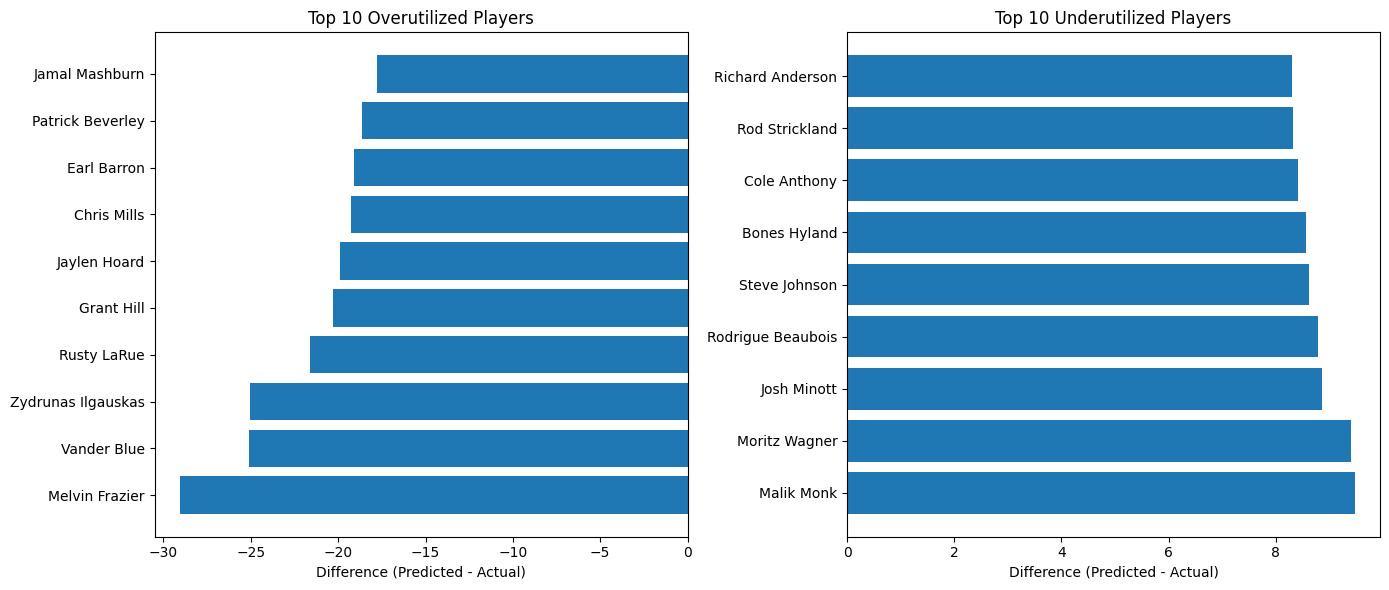
\includegraphics[width=0.8\textwidth]{MM_EP_TOP_TEN.png}
    \caption{Bar graph showing the top ten overutilized and underutilized players}
    \label{fig:minutes_decision_tree}
\end{figure}

Next, we decided to visualize team analytics instead of player analytics to better understand which NBA teams tended to over utilized or underutilized players that had low or high ideal numbers of minutes per game (MPG) respectively. This was based on the Random Forest Regressor model, which predicted the ideal MPG. After this, the difference between predicted and actual MPG was calculated for every team. A positive difference indicates teams that underutilized players (players who deserved more playtime) and a negative difference implies overutilized players (players who deserve less playtime). The results can be shown in a bar plot in the code, which shows that teams that were overutilizing players the most were the San Diego Sails (-5.71 mpg difference) and the Memphis Sounds (-2.08 mpg difference), and one of the teams that were underutilizing players the most were the Indiana Pacers (0.57 mpg difference).

\begin{figure}[H]
    \centering
    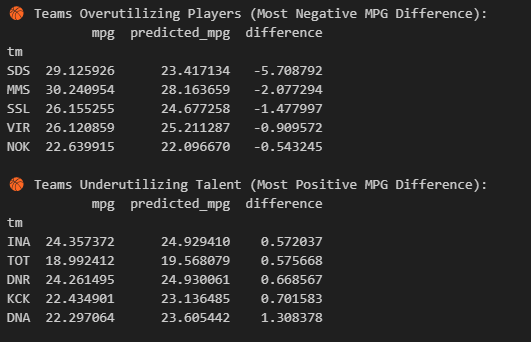
\includegraphics[width=0.8\textwidth]{MM_EP_TEAM_GRAPH.png}
    \caption{Table showing the teams overutilizing and underutilizing players}
    \label{fig:predicted_minutes_distribution}
\end{figure}

\begin{figure}[H]
    \centering
    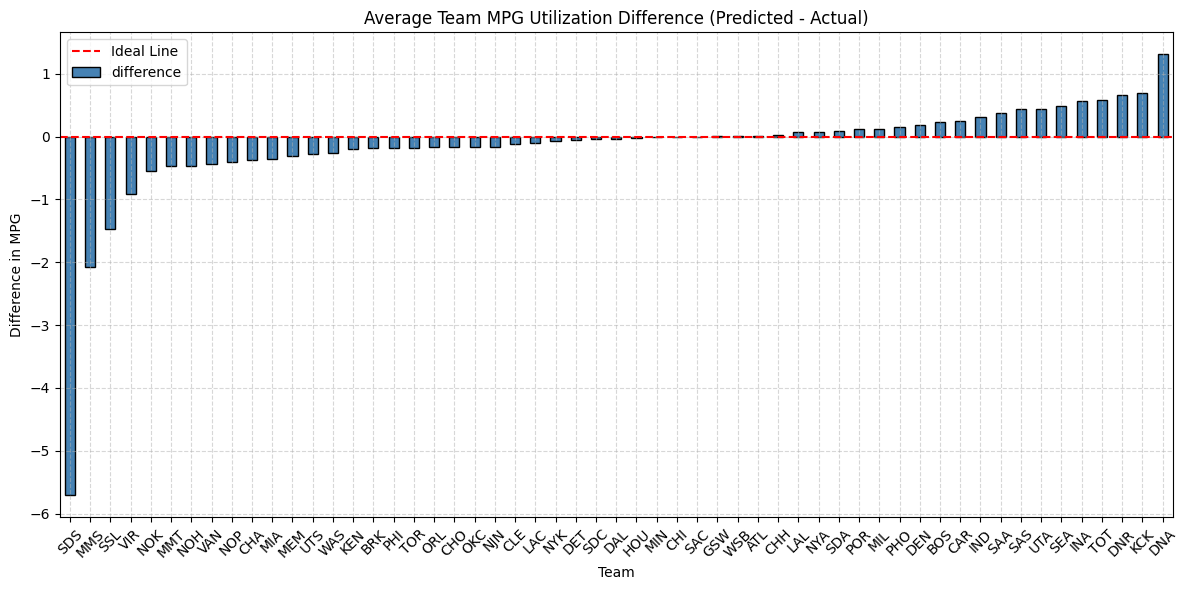
\includegraphics[width=0.8\textwidth]{MM_EP_TEAM_GRAPHIC_GRAPH.png}
    \caption{Bar plot showing the difference in minutes per game by team}
    \label{fig:team_minutes_analysis}
\end{figure}

\section{Conclusion and Potential Impact}
The study on NBA All-Star selections and player utilization demonstrates that machine learning algorithms, including logistic regression, random forests, and neural networks, can effectively predict All-Star selections and evaluate player utilization. By analyzing historical and current performance metrics, these models achieved high accuracy rates, with logistic regression reaching 92.22% accuracy in predicting All-Star selections. The models also produced strong R-squared values and low Root Mean Squared Errors for player utilization, indicating reliable predictions for identifying overutilized and underutilized players. However, the models have limitations in capturing certain nuances and intangibles. For instance, Grant Hill, a Hall of Famer, is flagged as overutilized by the model, which contradicts the consensus that a player of his caliber is rarely overutilized when leading their team. Similarly, Patrick Beverley, known for his defensive prowess and intangibles like physicality and leadership, is labeled as overutilized despite his value in guarding opposing stars, as his contributions are not fully reflected in traditional statistics. Despite these limitations, the models offer valuable insights into player utilization, aiding teams in making more informed decisions. The research also highlights key factors influencing All-Star selections, such as points, assists, and rebounds, and provides a framework for assessing player utilization by comparing predicted and actual minutes played. While the models are robust, they should be complemented with contextual understanding to account for intangibles and situational factors.

The findings have practical applications for NBA teams and analysts. By identifying underutilized players, teams can optimize their rosters, improving overall performance and for optimizing how player contracts are structured. Furthermore, the study highlights the importance of fairness and efficiency in All-Star voting and player utilization, ensuring that deserving players receive appropriate recognition and playing time.
In summary, this research highlights the potential of data-driven approaches to enhance decision-making in professional basketball, offering valuable tools for talent evaluation and team management.

\begin{thebibliography}{9}

\bibitem{wang2021}
Wang, Jingru, and Qishi Fan. “IOPscience.” \textit{Journal of Physics: Conference Series}, IOP Publishing, 1 Mar. 2021. Available: \url{https://iopscience.iop.org/article/10.1088/1742-6596/1802/3/032036}

\bibitem{georgievski2021}
Georgievski, Bojan, and Sabahudin Vrtagic. "Machine Learning and the NBA Game." \textit{Journal of Physical Education and Sport}, vol. 21, no. 6, 2021, pp. 3339–3343. Available: \url{https://www.researchgate.net/publication/363923964_Machine_learning_and_the_NBA_Game}

\bibitem{wang2023}
Wang, Junwen. "Predictive Analysis of NBA Game Outcomes through Machine Learning." \textit{Proceedings of the 5th International Conference on Machine Learning and Machine Intelligence}, 2023, pp. 1–6. Available: \url{https://dl.acm.org/doi/fullHtml/10.1145/3635638.3635646#bib11}

\bibitem{alonso2024}
Alonso, Fernando, and Davor Babac. "Evaluating the Effectiveness of Machine Learning Models for Predicting Basketball Game Outcomes." \textit{Knowledge and Information Systems}, 2024. Available: \url{https://link.springer.com/article/10.1007/s10115-024-02092-9}

\end{thebibliography}
\end{document}
